\section{Procedure}

In the procedure section a heuristic algorithm is provided for the Minimum Height Problem. Recall that the 
Minimum Height Problem asks, given some $\pi$ is there an algorithm for creating a minimal ladder 
from $MinL\{\pi\}$? Before providing the heuristic algorithm, it must be stated that there is an exact  
procedure to generate a minimal ladder from each $MinL\{\pi\}$ from $MinL\{\pi_{n}\}$. Refer to the minimal ladder for the reverse permutation 
of order $n$ as $MinL(Rev(\pi_{n}))$. In the introduction of this chapter, there 
is a description of a removal sequence of bars from $MinL(Rev(\pi_{n}))$ resulting in one  
minimal ladder for each $MinL\{\pi\}$ from $MinL\{\pi_{n}\}$. However, this method for creating a minimal ladder for an arbitrary 
permutation of order $n$ is inefficient. 
Using this method on some arbitrary permutation $\pi$ would first require creating $MinL(Rev(\pi_{n}))$, then each bar in $MinL(Rev(\pi_{n}))$ that 
does not correspond to an inversion in $\pi$ would need to be removed from the $MinL(Rev(\pi_{n}))$. 
The resulting ladder is a minimal ladder from $MinL\{\pi\}$. To see an example of the exact procedure 
for creating a minimal ladder, given some arbitrary $\pi$ of order $n$ please refer to Figure~\ref{Fig:ExactProcedure}. To see 
the algorithm for creating $MinL(Rev(\pi_{n}))$ please refer to Algorithm~\ref{Alg:MinRevLadder}.
\begin{center}
    \begin{figure}[h]
    \centering
    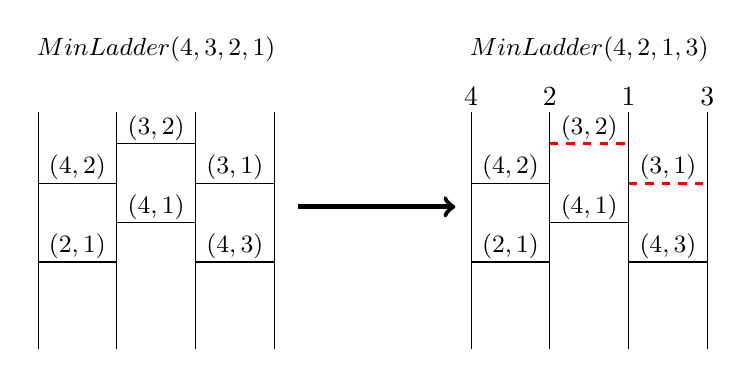
\begin{tikzpicture}
        \node at(7, 3.8){\small{$Min Ladder(4,3,2,1)$}};
        \draw(5.5, 0) to (5.5, 3);
            \draw(5.5, 2.1) to (6.5, 2.1);
            \draw(6.5, 1.6) to (7.5, 1.6);
            \draw(7.5, 1.1) to (8.5, 1.1);
        \draw(6.5, 0) to (6.5, 3);
            \draw(6.5, 2.6) to (7.5, 2.6);
            \draw(7.5, 2.1) to (8.5, 2.1);
        \draw(7.5, 0) to (7.5, 3);
            \draw(5.5, 1.1) to (6.5, 1.1);
        \draw(8.5, 0) to (8.5, 3);

        \node at(7, 2.8){\small{$(3,2)$}};
        \node at(8, 2.3){\small{$(3,1)$}};
        \node at(6, 2.3){\small{$(4,2)$}};
        \node at(7, 1.8){\small{$(4,1)$}};
        \node at(8, 1.3){\small{$(4,3)$}};
        \node at(6, 1.3){\small{$(2,1)$}};

        \draw[->, line width=.6mm](8.8, 1.8) to (10.8, 1.8);

        
        \node at(11, 3.2){4};
        \node at(12, 3.2){2};
        \node at(13, 3.2){1};
        \node at(14, 3.2){3};
        \node at(12.5, 3.8){\small{$Min Ladder(4,2,1,3)$}};

        \draw(11, 0) to (11, 3);
            \draw(11, 2.1) to (12, 2.1);
            \draw(12, 1.6) to (13, 1.6);
            \draw(13, 1.1) to (14, 1.1);
        \draw(12, 0) to (12, 3);
            \draw[red, dashed, line width = .4mm](12, 2.6) to (13, 2.6);
            \draw[red, dashed, line width = .4mm](13, 2.1) to (14, 2.1);
        \draw(13, 0) to (13, 3);
            \draw(11, 1.1) to (12, 1.1);
        \draw(14, 0) to (14, 3);

        
        \node at(12.5, 2.8){\small{$(3,2)$}};
        \node at(13.5, 2.3){\small{$(3,1)$}};
        \node at(11.5, 2.3){\small{$(4,2)$}};
        \node at(12.5, 1.8){\small{$(4,1)$}};
        \node at(13.5, 1.3){\small{$(4,3)$}};
        \node at(11.5, 1.3){\small{$(2,1)$}};
    \end{tikzpicture}
    \caption{Given $\pi=(4,2,1,3)$, the exact procedure first creates a min ladder for $(4,3,2,1)$ then removes bars to create a min ladder for $(4,2,1,3)$}
    \label{Fig:ExactProcedure}
\end{figure}
\end{center}

\subsection{Algorithm to create $MinL(Rev(\pi_{n}))$}
\begin{algorithm}
    \begin{algorithmic}[1]
        \Function{CMinRL}{$ladder$, $n$, $row$, $col$, $elem$}
            \If{\small{$elem = 0$ \textbf{OR} $elem = 1$}}
                \State \small{\textbf{return}}
            \EndIf
            \If{\small{$elem = n$}}
                \State \small{{\sc CMinRL}$(ladder, n, row \gets row+2, col \gets 1, elem \gets elem-2)$}
                \State \small{{\sc CMinRL}$(ladder, n, row \gets 1, col \gets 2, elem \gets elem-1)$}
            \Else 
                \If{\small{$n-elem = 2k$}}
                    \State \small{{\sc CMinRL}$(ladder, n, row \gets row+2, col \gets 1, elem \gets elem-2)$}
                \Else 
                    \State \small{{\sc CMinRL}$(ladder, n, row \gets 1, col \gets col+2, elem \gets elem-2)$}
                \EndIf
            \EndIf

        \State \small{$r \gets row, c \gets col$}
        \For{\small{$i$ \textbf{from} $1$ \textbf{to} $elem-1$}}
            \State \small{$ladder[r][c] \gets 1$}
            \State \small{$r \gets r+1,c \gets c+1$}
        \EndFor
        \EndFunction
    \end{algorithmic}
    \caption{Algorithm for creating $MinL(Rev(\pi_{n}))$}
    \label{Alg:MinRevLadder}
\end{algorithm}

Let $ladder$ be initialized to an empty two dimensional array. Let $n$ be initialized to $[n]$. Let $Row$ be initialized to 
$2$. Let $Col$ be initialized to $1$. Let $elem$ be initialized to $n$. The goal is to create $MinL(Rev(\pi_{n}))$.
The bars for the $nth$ element begin at $row=2$, 
$col=1$ and span to $row=2+(n-1)$, $col=(n-1)$. Each element equal to $n-2k$ where $0 \leq k \leq \lfloor(n/2)\rfloor$ indicates an element with the 
same polarity as $n$ and $\leq n$. We know from the introduction to this chapter that the routes of the same polarity as $n$ remain 
below the route of $n$. We also know that the first bar of each of these routes begins at column $1$.\par 
To calculate the row of the first bar of the $jth$ element where $j$ has the 
same polarity as $n$ consider the following. Let the previous element with the same polarity as $n$ be referred to as $j+2$.
Let the row of the first bar of the route of $j+2$ be equal to $m$. Thus, $ladder[m][1]$ is the first bar 
of the route of element $j+2$. We know that the second bar of the route of $j+2$ goes in $ladder[m+1][2]$. Thus, the 
first bar of the $jth$ route must begin at $row=m+2$; it cannot go in $ladder[m][1]$ seeing as the first bar 
of $j+2$ occupies this cell. Nor can it go in $ladder[m+1][1]$ seeing as the second bar of the route of $j+2$ 
is at $ladder[m+1][2]$. Nor can it go in a $row > m+2$ seeing as the ladder would no longer be minimal. Thus, 
the first bar of the route of element $j$ is at $ladder[m+2][1]$ where $m$ is the row of the first bar of the route 
of element $j+2$.\par 
Each element equal to $n-(2k+1)$  where $0 \leq k \leq \lfloor(n/2)\rfloor$ indicates an element with the opposite polarity as $n$ and $\leq n$. We know 
from the introduction to this chapter that the routes of elements with the opposite polarity of $n$ are right swapped above the routes 
of all elements greater than themselves. We also know from the introduction that the first 
bar of each of these routes begin at row $1$ in $MinL(Rev(\pi_{n}))$. The number of bars in each of these elements' 
routes equals $j-1$ where $j$ is one of these elements. Lastly, we know from the introduction of this chapter, that the last 
bar of each of these elements' routes end at column $n-1$/the last column in $ladder$.\par 
To calculate the column of the first bar of the $jth$ element where $j$ has the opposite polarity 
as $n$ consider the following. Let the previous element with the opposite polarity as $n$ be referred to as $j+2$. 
Let the column of the first bar of the route of $j+2$ be equal to $m$. Thus, $ladder[1][m]$ is the first bar 
of the route of element $j+2$. We know that the first bar of the route of element $j$ must begin at row $1$. 
This bar cannot go in $ladder[1][m]$ seeing as this is where the first bar of the route of element $j+2$. 
Nor can this bar go in $ladder[1][m+1]$ seeing as if it did, its left endpoint would be touching the right 
endpoint of the first bar of the route of element $j+2$. Nor can it go in $ladder[1][m+>2]$ seeing as if it 
did, the bars of route $j$ would extend beyond the last/$n-1th$ column in $ladder$. 
\begin{lemma}
    The column for the first bar of element $j's$ route is $m+2$.
    
\end{lemma}
\begin{proof}
    \begin{itemize}
        \item     Let the column of the first bar of element $j+2's$ route be $m$. 
        \item     Let the number of columns in $ladder=n-1$.
        \item     Let the number of bars in $j+2's$ route be equal to $j+2-1=j+1$.
    \end{itemize}
        From the axioms we get the equation $n-1-(j+1)=m$.
        We need to derive $n-1-(j-1)=m+2$ from $n-1-(j+1)=m$.
   \begin{equation} \label{eq1}
        \centering
        \begin{split}
            (n-1)-(j+1)=m \\
            (n)-(j)= m+2\\
            (n-1)-(j)=m+2-1=m+1 \\ 
            (n-1)-(j-1)=m+2-1+1=m+2\\
            (n-1)-(j-1) = m+2\\
        \end{split}
    \end{equation}
   Thus, the first bar for $j's$ route is $m+2$.
   To see $MinL((5,4,3,2,1))$ please refer to Figure~\ref{Fig:RootToMinLadder}.
\end{proof}


\begin{lemma}
    The time complexity of $CMinRL$ is $O{n \choose 2}$ 
\end{lemma}
\begin{proof}
    For each element, $x$, in $Rev(\pi_{n})$, the function makes a recursive call and the function 
    adds all $x-1$ bars belonging to $x's$ route in the ladder. The total number of bars for the $MinL(Rev(\pi))$
    equals the number of inversions for $Rev(\pi_{n})$ which is equal to ${n \choose 2}$. 
\end{proof}



\subsection{The Heuristic Algorithm to create $MinL(\pi)$}

In the previous section, the algorithm to create $MinL(Rev(\pi))$ was provided.\newline {\sc CMinRL}
is exact, but unfortunately only creates the minimal ladder for the reverse permutation. The following algorithm 
is a heuristic algorithm for creating a minimal ladder for any permutation. The heuristic algorithm 
is based on inserting the maximum the number of bars per row of the ladder. Each bar uninverts and inversion, 
two or more bars on the same row uninvert two or more inversions in parallel. Thinking back to sorting networks, 
when two or more connectors are directly above/below each other, the connectors swap elements in tandem. The same 
can be said for bars on the same row of the ladder.
One can say if a ladder has a height of 
one, then it sorts $\pi$ into $\pi_{ID}$ in one step. If a ladder has a height of two, then it sorts $\pi$ into an intermediary $\pi_{2}$
in row $1$ then sorts $\pi_{2}$ into $\pi_{ID}$ in row $2$, etc.
Define \emph{bar compression} as the average number of bars per row in a ladder; if the ladder has zero rows and/or zero bars, then the 
bar compression is undefined. The more bars per row the higher the bar compression, the less bars per row the lower the bar compression. The heuristic algorithm 
works by maximizing bar compression of a ladder. It should be intuitive that given a ladder with $b$ bars, 
each bar could be given its own row; in this case the ladder would have the least bar compression. This ladder 
is the opposite of the minimal ladder. Thus, for the heuristic algorithm, the goal is to squeeze as many bars in the same row as possible in 
order to maximize the bar compression of a ladder.\par 
Recall that when inverted elements of $\pi$ travel through the ladder and cross a bar, the elements are swapped, thus resulting in 
some intermediate permutation $\pi_{k}$. Define $InvPi(\pi)$ as the permutation of intermediate permutations, beginning at $\pi$ and 
ending at the identity permutation. Each $\pi_{k} \in InvPi(\pi)$ corresponds to a row from a unique $ladder \in OptL\{\pi\}$. 
Given some arbitrary $\pi$, there can be more than one $InvPi(\pi)$. See table~\ref{Tab:InvPi}. 
for two different $InvPi(3,5,4,6,2,1)$.

\begin{table}[!htp]
    \begin{tabular}{|p{3cm}|p{5cm}|p{5cm}|}
        \hline 
    \multicolumn{3}{|c|}{2 $InvPi(3,5,4,6,2,1)$}\\
    \hline 
    \hline 
    $\pi_{k}$ & $A=InvPi(3,5,4,6,2,1)$ & $B=InvPi(3,5,4,6,2,1)$\\ 
    \hline 
    $\pi_{1}$ & $(3,5,4,6,2,1)$ & $(3,5,4,6,2,1)$\\ 
    \hline
    $\pi_{2}$ & $(3,4,5,6,1,2)$ & $(3,4,5,6,2,1)$\\ 
    \hline 
    $\pi_{3}$ & $(3,4,5,1,6,2)$ & $(3,4,5,2,6,1)$ \\ 
    \hline 
    $\pi_{4}$ & $(3,4,1,5,2,6)$ & $(3,4,2,5,6,1)$ \\ 
    \hline 
    $\pi_{5}$ & $(3,1,4,2,5,6)$ & $(3,2,4,5,1,6)$\\ 
    \hline 
    $\pi_{6}$ & $(1,3,2,4,5,6)$ & $(2,3,4,1,5,6)$\\ 
    \hline 
    $\pi_{7}$ & $(1,2,3,4,5,6)$ & $(2,3,1,4,5,6)$\\ 
    \hline 
    $\pi_{8}$ & $none$  & $(2,1,3,4,5,6)$ \\ 
    \hline 
     $\pi_{9}$ & $none$  & $(1,2,3,4,5,6)$ \\ 
    \hline 

        
    \end{tabular}
    \caption{Table for two different InvPi(3,5,4,6,2,1)}
    \label{Tab:InvPi}
\end{table}



When creating a $MinL(\pi)$, the goal is to create a ladder with the least number of rows, which in turn corresponds 
to the shortest $InvPi(\pi)$.
Let $MinInvPi(\pi)$ be the $InvPi(\pi)$ generated by the heuristic algorithm.
Let $\pi^{k} \in MinInvPi(\pi)$. Then the recurrence relation for \begin{small}$\pi^{k}=\pi^{k-1} \rightarrow \tau(p^{k-1}_{i},p^{k-1}_{i+1}) | p^{k-1}_{i}>p^{k-1}_{i+1}$ $\mbox{ and for any }$$\tau(\pi^{k-1}_{i},\pi^{k-1}_{i+1}) \cap \tau(\pi^{k-1}_{j},\pi^{k-1}_{j+1}) = \emptyset$.\end{small}
In simpler terms, for some $\pi^{k} \in MinInvPi(\pi)$, perform the maximum number 
of adjacent transpositions on adjacent inversions in $\pi^{k-1}$ as is possible.
In turn, this means the maximum number of bars can be added to the $kth$ row in the ladder.
The less rows there are in the ladder the smaller the corresponding 
 $InvPi(\pi)$ and the greater the bar compression.
 To see an example of maximal bar compression and a corresponding $MinInvPi(\pi)$, please refer to Figure~\ref{Fig:BarCompressionInvPi}.

\begin{figure}[!htp]
    \begin{minipage}{.45\textwidth}
        \centering 
    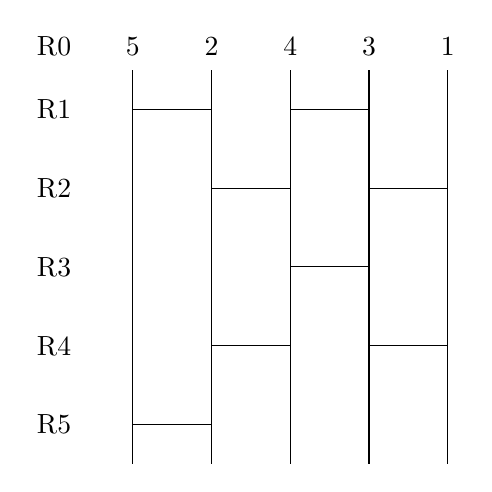
\begin{tikzpicture}
        \node at (0, 5.3)(a){5};
        \node at (1, 5.3)(b){2};
        \node at (2, 5.3)(c){4};
        \node at (3, 5.3)(d){3};
        \node at (4, 5.3)(e){1};

        \draw(0, 0) to (0, 5);
            \draw(0, 4.5) to (1, 4.5);
            \draw(1, 3.5) to (2, 3.5);
            \draw(2, 2.5) to (3, 2.5);
            \draw(3, 1.5) to (4, 1.5);
        \draw(1, 0) to (1, 5);
            \draw(2, 4.5) to (3, 4.5);
            \draw(3, 3.5) to (4, 3.5);
        \draw(2, 0) to (2, 5);
            \draw(0, .5) to (1, .5);
            \draw(1, 1.5) to (2, 1.5);
        \draw(3, 0) to (3, 5);
        \draw(4, 0) to (4, 5);



        \node at(-1, 5.3){R0};
        \node at(-1, 4.5){R1};
        \node at(-1, 3.5){R2};
        \node at(-1, 2.5){R3};
        \node at(-1, 1.5){R4};
        \node at(-1, 0.5){R5};
    \end{tikzpicture}
    \end{minipage}
       \begin{minipage}{.45\textwidth}
        \centering 
    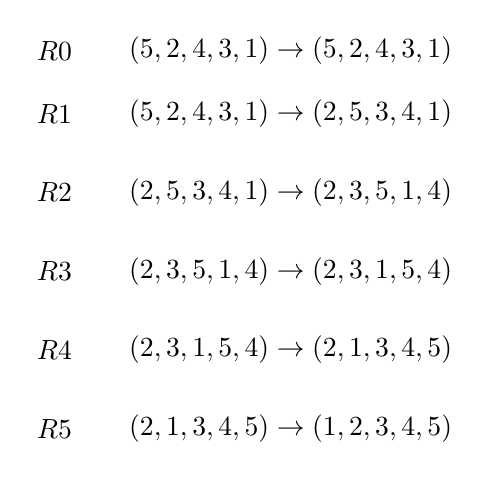
\begin{tikzpicture}
        \draw node at(0, 5.5){$(5,2,4,3,1) \rightarrow (5,2,4,3,1)$};
      \draw node at(0, 4.7){$(5,2,4,3,1)\rightarrow (2,5,3,4,1)$};
      \draw node at(0, 3.7){$(2,5,3,4,1) \rightarrow (2,3,5,1,4)$};
      \draw node at(0, 2.7){$(2,3,5,1,4) \rightarrow (2,3,1,5,4)$};
      \draw node at(0, 1.7){$(2,3,1,5,4) \rightarrow (2,1,3,4,5)$};
      \draw node at(0, 0.7){$(2,1,3,4,5) \rightarrow (1,2,3,4,5)$};
      \node at(-3, 5.5){$R0$};
      \node at(-3, 4.7){$R1$};
      \node at(-3, 3.7){$R2$};
      \node at(-3, 2.7){$R3$};
      \node at(-3, 1.7){$R4$};
      \node at(-3, .7){$R5$};
    \end{tikzpicture}
    \end{minipage}
    
    \caption{The ladder on the left has a bar compression of $8/5$. The corresponding $InvPi((5,2,4,3,1))$ is on the right.}
    \label{Fig:BarCompressionInvPi}
    
\end{figure}
\pagebreak


%%%%%%%%%%%%%%FIX ME%%%%%%%%%%%%%%%%%%%%%%%%%%%%%%%%%%%%

The following algorithm is a heuristic algorithm for creating a minimal ladder for 
any arbitrary permutation of order $n$. Let $ladder$ be initialized 
to an $n$ by $n-1$ empty two dimensional array. Let $row$ be initialized 
to $1$. Let $\pi$ be an arbitrary permutation of order $n$. The algorithm consists 
of two functions. One is {\sc HeuristicMinLadder} and the other is {\sc PreProcessRowOne}.
Define a \emph{decreasing substring of $\pi$ (DSS for short)}
as follows: given some value $k$ $2 \leq k \leq n$, a decreasing substring of length $k$ is defined as $p_{i}>\pi_{i+1}>\pi_{i+2} \dots > \pi_{k}$.
A DSS in $\pi$ can 
be even or odd; the polarity of the DSS is defined by the length of the substring. For example, 
the DSS $(3,2,1)$ has odd polarity whereas the DSS $(4,3,2,1)$ has even polarity. A DSS terminates when ceases to be an adjacent inversion. 
For example, given $(3,2,1,4)$ in $\pi$, the DSS is $(3,2,1)$ which 
has odd polarity. Let $S$ be the set of all $DSS_{2k} \in \pi$.
Let $T$ be the set of all $DSS_{2k+1} \in \pi$.
$S$ and $T$ are only used in {\sc PreProcessRowOne}.
\emph{Maximal zig-zagginess} is defined as follows:
\begin{small}
\begin{caseof}
    
    Max zig-zag = 
        $\begin{cases}
            p_{1} < p_{2} > p_{3} < p_{4} \dots p_{n-1=2k} > p_{n=2k+1} & \mbox{if } n=2k+1 \mbox{ and } p_{1} < p_{2}\\
            p_{1} > p_{2} < p_{3} > p_{4} \dots  p_{n-1=2k} < p_{n=2k+1} & \mbox{if } n=2k+1 \mbox { and } p_{1} > p_{2}\\ 
            p_{1} < p_{2} > p_{3} < p_{4} \dots p_{n-1=2K-1} < p_{n=2k} & \mbox{if } n=2k \mbox{ and } p_{1} < p_{2}\\ 
            p_{1} < p_{2} > p_{3} < p_{4} \dots p_{n-1=2K-1} < p_{n=2k} & \mbox{if } n=2k \mbox{ and } p_{1} > p_{2}\\
        \end{cases}$
   
\end{caseof}
 \end{small}\pagebreak

\begin{algorithm}[!htp]
        \begin{algorithmic}[1]
            \Function{HeuristicMinLadder}{$ladder$, $\pi$, $n$, $row$}
                \If{\small{{\sc Sorted}$(\pi)$}}
                    \State \small{\textbf{return}}
                \EndIf
                \If{\small{$row = 1$}}
                    \State \small{$\pi_{2} \gets$ {\sc PreProcessRowOne}$(\pi,n)$}
                    \For{$i$ \textbf{from} $1$  \textbf{to} $n$}
                        \If{\small{$p_{i} \neq \pi'_{i}$}}
                            \State \small{$ladder[1][i] \gets 1$}
                            \State \small{$i \gets i+1$} 
                        \EndIf
                    \EndFor
                    \State $\pi \gets \pi_{2}$
                    \State $row \gets row+1$
                    \State \small{{\sc HeuristicMinLadder}$(Ladder, \pi, n, row)$}
                \Else
                    \For{\small{$i$ \textbf{from} $1$, \textbf{to} $n-1$}}
                        \If{\small{$p_{i}>\pi_{i+1}$}} 
                            \State \small{{\sc Swap}$(\pi{i}, \pi_{i+1})$}
                            \State \small{$ladder[row][i] \gets 1$}
                            \State \small{$i \gets i+1$}
                        \EndIf
                    \EndFor
                    \State \small{{\sc HeuristicMinLadder}$(ladder, \pi, n, row \gets  row+1)$}
                \EndIf
            \EndFunction
        \end{algorithmic}
        \caption{Heuristic algorithm to create a ladder with minimal height}
        \label{Algo:heuristic}
    \end{algorithm}\pagebreak
    \begin{algorithm}[!htp]
         \begin{algorithmic}[1]
            \Function{PreProcessRowOne}{$\pi$, $n$, $S$, $T$}
                \State \small{$\pi_{a} \gets \pi$}
                \State \small{$\pi_{b} \gets \pi$}
                \For {\textbf{each} $DSS_{2k}\in S$}
                    \State $\tau(pa_{i},pa_{i+1}),\tau(pa_{i+2},pa_{i+3}) \dots \tau(pa_{i+2k-2},pa_{i+2k-1}$ 
                    \State $\tau(pb_{i},pb_{i+1}),\tau(pb_{i+2},pb_{i+3}) \dots \tau(pb_{i+2k-2},pb_{i+2k-1}$ 
                    \State \small{Where $\tau(pa_{i},pa_{i+1})$/$\tau(pb_{i},pb_{i+1})$ uninverts an adjacent 
                    inversion in $\pi_{a}/\pi_{b}$ corresponding to the inversion in the $DSS_{2k} \in S$}
                \EndFor
                \For {\textbf{each} $DSS_{2k+1}\in T$}
                    \State From left to right $\tau(pa_{i},pa_{i+1}),\tau(pa_{i+2},pa_{i+3}) \dots \tau(pa_{i+2k-2},pa_{i+2k-1})$
                    \State \small{Where $\tau(pa_{i},pa_{i+1})$ uninverts an adjacent 
                    inversion in $\pi_{a}$ corresponding to the inversion in the $DSS_{2k+1}\in T$}
                \EndFor
                \For {\textbf{each} $DSS_{2k+1}\in T$}
                    \State From right to left $\tau(pb_{i},pb_{i-1}),\tau(pb_{i-2},pb_{i-3}) \dots \tau(pb_{i-2k-3},pb_{i-2k-2})$
                    \State \small{Where $\tau(pb_{i},pb_{i-1})$ uninverts an adjacent 
                    inversion in $\pi_{b}$ corresponding to the inversion in the $DSS_{2k+1}\in T$}
                \EndFor
                \If{\small{$\pi_{a}$ and $\pi_{b}$ are equally zig-zaggy}}
                    \State return $\pi_{b}$
                \ElsIf{$\pi_{a}$ is more zig-zaggy than $\pi_{b}$}
                    \State \textbf{return $\pi_{a}$}
                \Else 
                    \State \textbf{return $\pi_{b}$}
                \EndIf

            \EndFunction
        
        \end{algorithmic} 
        \caption{Algorithm to return the second permutation from $InvPi(\pi)$ which will result in the maximal bar compression}
        \label{Algo:PreProcessRow}
\end{algorithm}\pagebreak

The more zig-zaggy the resulting permutation from {\sc PreProcessRowOne} is, the more bars are added 
to row $1$ of the ladder. {\sc PreProcessRowOne} returns the $\pi_{2}$ from some $MinInvPi(\pi)$; the first permutation being $\pi_{1}=\pi$. 
There are two criteria for $\pi_{2}$. The first is $\pi_{2}$ is a transformation of $\pi$ such that $\pi$ 
has undergone as many adjacent transpositions as possible.
The second criteria for $\pi_{2}$ is that $\pi_{2}$ is as zig-zaggy as possible, given that it has undergone the maximum amount of 
adjacent transpositions. When a DSS is of even length, then there are $k/2$ adjacent inversions that can be uninverted in tandem, 
where $k$ is the length of the DSS. 
For example, given DSS $(4,3,2,1)$, $\tau(4,3)$ and $\tau(2,1)$ are done in tandem. When a DSS is of odd length, the maximum 
number of adjacent inversions that can be uninverted in tandem is $\lfloor(k/2)\rfloor$ where $k$ is the length of the DSS. A choice 
needs to be made in terms of whether or not the first element in the DSS will be transposed or the $kth$ element in the substring will be 
transposed. For example, given the DSS $(5,4,3,2,1)$, either $\tau(5,4),\tau(3,2)$ or $\tau(4,3)\tau(2,1)$ are legitimate options. 
The first step of {\sc PreProcessRowOne} is to perform  $k/2$ $\tau(p_{i},p_{i+1})$ in tandem for all
even length $DSS \in S$. Then, for all odd length $DSS \in T$,
 {\sc PreProcessRowOne} performs $\lfloor k/2\rfloor$ $\tau(pa_{i}, pa_{i+1}), \dots \tau(pa_{k-2},pa_{k-1})$
resulting in a candidate permutation $\pi_{a}$. {\sc PreProcessRowOne} then performs 
$\lfloor k/2 \rfloor$ $\tau(pb_{k},pb_{k-1}) \dots \tau(pb_{3},pb_{2})$
resulting in a second candidate permutation $\pi_{b}$.
This results in two candidate permutations for $\pi_{2}$ in $MinInvPi(\pi)$. 
In order to choose between $\pi_{a}$ and $\pi_{b}$, 
the algorithm then checks for which of the two have a better zig-zag pattern; a better zig-zag 
pattern is a relation between two permutations such that if one permutation is closer to maximal zig-zagginess 
than the other, then it has a better zig-zag pattern. The reason the algorithm looks 
for better zig-zagginess is because the more zig-zaggy a permutation is, the more adjacent
$2$ length DSS there are in said permutation. The more adjacent $2$ lengthed DSS there are, 
the more pairwise disjoint adjacent inversions there are in said permutation. 
The more pairwise disjoint adjacent 
inversions there are in a permutation, the more bars can be added to ladder at the row corresponding to the permutation. 
The result is likely to be $MinL(\pi)$ and the shortest length $InvPi(\pi)$. 
Once $\pi_{2}$ has been selected from {\sc PreProcessRowOne}, 
{\sc HeuristicMinLadder} adds the corresponding bars to the ladder. Then, {\sc HeuristicMinLadder}
continues to perform the maximal number $\tau(p_{i},p_{i+1})$ in each 
subsequent $\pi_{k}$ until $\pi_{k}=\pi_{ID}$. {\sc HeuristicMinLadder} adds bars 
to the $kth$ row accordingly. If any intermediate $\pi_{k}$  has a $DSS_{2k+1}$ then 
{\sc HeuristicMinLadder} swaps from left to right. To see $MinL((3,9,8,4,1,2,5,7,6))$ please refer to 
Figure~\ref{Fig:MinLadder}.
To see an example 
of the resulting $pi_{2}$ from {\sc PreProcessRowOne} given $\pi=(4,3,9,8,7,6,12,11,5,2,1,14,13,10)$ please refer to Example~\ref{Example:PreProcessRowOne}.


%%%%%%%%%%%%%%%%%FIGURE FOR MINL%%%%%%%%%%%%%%%%%%%%
\begin{figure}
    \centering
    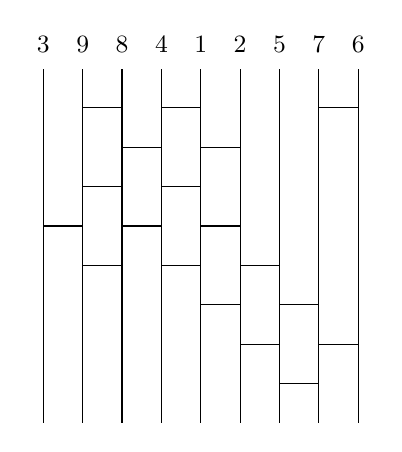
\begin{tikzpicture}
        \draw(0,1.5) to (0,6);
        \draw(.5,1.5) to (.5,6);
        \draw(1,1.5) to (1,6);
        \draw(1.5,1.5) to (1.5,6);
        \draw(2,1.5) to (2,6);
        \draw(2.5,1.5) to (2.5,6);
        \draw(3,1.5) to (3,6);
        \draw(3.5,1.5) to (3.5,6);
        \draw(4,1.5) to (4,6);

        \node at(0, 6.3){\small{$3$}};
        \node at(.5, 6.3){\small{$9$}};
        \node at(1, 6.3){\small{$8$}};
        \node at(1.5, 6.3){\small{$4$}};
        \node at(2, 6.3){\small{$1$}};
        \node at(2.5, 6.3){\small{$2$}};
        \node at(3, 6.3){\small{$5$}};
        \node at(3.5, 6.3){\small{$7$}};
        \node at(4, 6.3){\small{$6$}};

        \draw(0.5,5.5) to (1, 5.5); \draw(1.5,5.5) to (2,5.5); \draw(3.5,5.5) to (4, 5.5);
        \draw(1,5.0) to (1.5, 5.0); \draw(2,5.0) to (2.5, 5.0); 
        \draw(.5,4.5) to (1, 4.5); \draw(1.5,4.5) to (2, 4.5); 
        \draw(0,4.0) to (0.5, 4.0); \draw(1,4.0) to (1.5, 4.0); \draw(2,4.0) to (2.5, 4.0);
        \draw(0.5,3.5) to (1, 3.5); \draw(1.5,3.5) to (2, 3.5); \draw(2.5,3.5) to (3, 3.5);
        \draw(2,3) to (2.5, 3); \draw(3,3) to (3.5, 3);
        \draw(2.5,2.5) to (3, 2.5); \draw(3.5,2.5) to (4, 2.5);
        \draw(3,2.0) to (3.5, 2.0); 

    \end{tikzpicture}
    \caption{The resulting ladder from {\sc HeuristicMinLadder}}
    \label{Fig:MinLadder}
\end{figure}


\begin{example} 
    Example demonstrating {\sc PreProcessRowOne}
    \begin{enumerate}
        \item Let  $\pi=(4,3,9,8,7,6,12,11,5,2,1,14,13,10)$
        \item Let $S=\{(4,3),(9,8,7,6)\}$
        \item Let $T=\{(12,11,5,2,1),(14,13,10)\}$
        \item Step 1: {\sc PreProcessRowOne} assigns $\pi$ to two candidate permutations $\pi_{a}$ and $\pi_{b}$.
        \item Step 2: Perform adjacent transpositions for each $DSS \in S$ in $\pi_{a},\pi_{b}$.
        \item After applying step 2: $\pi_{a}=(3,4,8,9,6,7,12,11,5,2,1,14,13,10)$ 
        \item After applying step 2: $\pi_{b}=(3,4,8,9,6,7,12,11,5,2,1,14,13,10)$ 
        \item Step 3a): Perform adjacent transpositions for each $DSS \in T$ in $\pi_{a}$ going left 
        to right beginning at the leftmost element of each $DSS \in T$.
        \item After applying step 3a: $\pi_{a}=(3,4,8,9,6,7,11,12,2,5,1,13,14,10)$
        \item Step 3b): Perform adjacent transpositions for each $DSS \in T$ in $\pi_{b}$ going right 
        to left beginning at the rightmost element of each $DSS \in T$.
        \item After applying step 3b: $\pi_{b}=(3,4,8,9,6,7,12,5,11,1,2,14,10,13)$.
        \item Calculate the zig-zagginess for $\pi_{a}=13-(2+2+1)=8$.
        \item Calculate the zig-zaginess for $\pi_{b}=13-(2+1+1)=9$.
        \item $\pi_{b}$ is more zig-zaggy than $\pi_{a}$. Therefore return $\pi_{b}$.
    \end{enumerate}
    End of example.
    \label{Example:PreProcessRowOne}
\end{example}

The zig-zagginess of a permutation is calculated as follows. Given $n$ elements in $\pi$ there 
are $n-1$ adjacent relations between the $n$ elements in $\pi$ such that either $\pi_{i}>\pi_{i+1}$
or $\pi_{i}<\pi_{i+1}$. Refer to the gap between two elements in $\pi$ as \emph{spots in the permutation}. Thus, 
there are $n-1$ spots in the permutation such that each spot can take on the $>$ or $<$ relation. 
If a permutation is maximally zig-zaggy, then for any two spots, $s_{j-1}$, $s_{j}$
if $s_{j-1}$ is $<$ then $s_{j}$ is $>$ and if $s_{j-1}$ is $>$ then $s_{j}$ is $<$.
Therefore, a permutation with maximal zig-zagginess has a zig-zagginess value of $n-1$.
Whenever there is an $s_{j-1}$ that has the same relation as $s_{j}$ subtract $1$ from 
$n-1$. I.E. if $s_{j-1}$ is $<$ and $s_{j}$ is $<$ then subtract $1$ from $n-1$. The resulting 
number is the value of the zig-zagginess of $\pi$. In the above example, $(n-1)=13$, 
$\pi_{a}$ has a zig-zagginess of $13-5=8$ and $\pi_{b}$ has a zig-zagginess of $13-4=9$. 
Therefore, $\pi_{b}$ is used as $\pi_{2}$ in $MinInvPi((4,3,9,8,7,6,12,11,5,2,1,14,13,10))$.

\begin{lemma}
    Given $j$ adjacent inversions in $\pi_{k}$, the more of these inversions that are pairwise disjoint, the more 
    bars can be added to the $kth$ row.
\end{lemma}
\begin{proof}
    We shall use proof by induction. Let $m$ be the number of elements it takes to create $j$ adjacent inversions.
    Let $n$ be the number of bars that can be added to the $kth$ row of ladder.
    Inductive Hypothesis:\newline

    m,n=:$\begin{cases}
            2j,j \small{\mbox{ if j adjacent inversions are pairwise disjoint}}\\
            j+1,\lceil(j/2)\rceil \small{\mbox{ if j adjacent inversions are not pairwise disjoint.}}\\\small{\mbox{Bars added right to left}}\\
            j+1,\lfloor(j/2)\rfloor \small{\mbox{ if j adjacent inversions are not pairwise disjoint.}}\\\small{\mbox{Bars added left to right}}\\
        \end{cases}$\\



    Base case 1: let $\pi=(4,3,2,1)$/$j=2$. $(4,3) \cap (2,1) = \emptyset$ and $m=2j=4$ and $n=2=j$. \newline 
    Base case 2: let $\pi=(3,2,1)$/$j=2$. $(3,2) \cap (2,1)= \{2\}$ and $m=j+1=3$ and $n=1=\lceil(j/2)\rceil$.\newline
    Base case 3: let $\pi=(3,2,1)$/$j=2$. $(3,2) \cap (2,1)= \{2\}$ and $m=j+1=3$ and $n=1=\lfloor(j/2)\rfloor$.\newline



    We need to show that for $j+1$, $m=2(j+1)$ and $n=j+1$ when the $j+1th$ adjacent inversion is pairwise disjoint.
    We also need to show that for $j+1$, $m=j+1+1$ and $n=\lceil(j+1/2)\rceil/\lfloor(j+1/2)\rfloor$ when the $j+1th$ adjacent inversion is not pairwise 
    disjoint.\par



    Suppose the $j+1th$ adjacent inversion is pairwise disjoint and suppose the first $j$ adjacent inversions are also 
    pairwise disjoint, then this would require two more elements to form an 
    inversion in $\pi$. The reason being is that if the $j+1th$ inversion was formed by one more element in $\pi$ then 
    the $j+1th$ inversion would not be pairwise disjoint. Let this element be referred to as $x$. We shall prove by contradiction 
    that if $x$, on its own, forms the $j+1th$ adjacent inversion in $\pi$ then inversion $j+1$ cannot be pairwise disjoint. Let $inv(a,b)$ 
    be the $jth$ inversion in $\pi$ where $a>b$. If one were to insert $x$
    to the left $a$ and $x>a$ then $inv(x,a) \cap inv(a,b) \neq \emptyset$. If one were to insert $x$ to the right of $b$ and 
    $x<b$ then $inv(a,b) \cap inv(b,x) \neq \emptyset$. Therefore, we have a contradiction. Thus, if adjacent inversion $j+1$ 
    is a pairwise disjoint, then $2$ more 
    elements are required to make the $j+1th$ adjacent inversion. Therefore, $m=2(j+1)=2j+2$ where the $+2$ accounts for the 
    two more elements required to make the $j+1th$ inversion. $n=j+1$ seeing as $j$ inversions are pairwise disjoint, then the $j$ bars 
    at row $k$ in $ladder$ are at least two columns away from every other bar corresponding 
    to one of the $j$ inversions. Since the $j+1th$ adjacent inversion is also pairwise disjoint from all other $j$ inversions, 
    then the bar corresponding to this inversion is 
    also placed at least two columns away from the other bars in the $kth$ row. Thus, $n=j+1$.\par 


    Suppose the $j+1th$ adjacent inversion is not pairwise disjoint and suppose the first $j$ inversions 
    are also not pairwise disjoint, then the $j+1th$ adjacent inversion would require one more element to form an inversion 
    in $\pi$. We shall do a direct proof to show that one more element is required. Let $inv(a,b)$ be the $jth$ inversion 
    in $\pi$ where $a>b$. Let $x$ be the element to form the $j+1th$ inversion in $\pi$. If one were to insert $x$
    to the left $a$ and $x>a$ then $inv(x,a) \cap inv(a,b) \neq \emptyset$.  If one were to insert $x$ to the right of $b$ and 
    $x<b$ then $inv(a,b) \cap inv(b,x) \neq \emptyset$. Therefore, in both cases, when $x$ forms the $j+1th$ inversion, 
    the $j+1th$ inversion is not pairwise disjoint, which is exactly what we are trying to prove. Since the $xth$ element 
    forms the $j+1th$ inversion then $m=j+1+1=j+2$ where the additional $+1$ comes from the $xth$ forming the $j+1th$ inversion.\par 

    Next, suppose that $a$ is  the leftmost element of the first $j$ inversions. Let the position of $a$ in $\pi=i$. 
    Thus, $p_{i}=a$.  
    Also, suppose that the first $j/2$ bars are added to $row=k$ going left to right and element $x$ is directly to the left of $a$ 
    in $\pi$ forming  the $j+1th$ inversion. 
    Seeing as element $p_{i}$ and $p_{i+1}$ have a bar on row $k$ then elements $x$ and $a$ cannot have a bar on row $k$, 
    thus $n=\lfloor(j+1/2)\rfloor$. Next, suppose that the first $j/2$ bars are added to $row=k$ going right to left, then it is possible to place a 
    bar on row $k$ for elements $x$ and $a$, thus $n=\lceil(j+1/2)\rceil$. Next suppose that $b$ is the rightmost element for the first 
    $j$ inversions. Let the position of $b$ in $\pi=l$. Thus, $p_{l}=b$. Also, suppose that the first $j/2$ bars are added to 
    $row=k$ going right to left and element $x$ is directly to the right of $b$ in $\pi$ forming the $j+1th$ inversion.
    Seeing as element $p_{l-1}$ and $p_{l}$ have a bar on row $k$ then elements $x$ and $b$ cannot have a bar on row $k$, 
    thus $n=\lfloor(j+1/2)\rfloor$.
    Next, suppose that the first $j/2$ bars are added to $row=k$ going left to right, then it is possible to place a 
    bar on row $k$ for elements $x$ and $b$, thus $n=\lceil(j+1/2)\rceil$.

    Clearly $n=j>n=\lfloor(j/2)\rfloor/\lceil(j/2)\rceil$, therefore, the more adjacent inversions that are pairwise disjoint, the more bars 
    can be added to $ladder$ in row $k$.
    To see an example of the above proof please refer to Figure~\ref{Fig:PairwiseDisjoint}.

\end{proof}\pagebreak


\begin{figure}[t]
    \centering
    \begin{minipage}{.9\textwidth}
        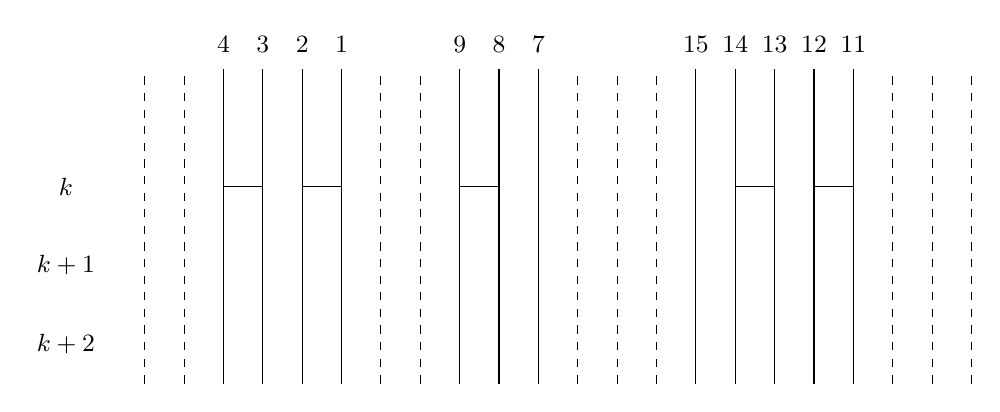
\begin{tikzpicture}
            \draw[dashed](0, 0) -- (0, 4);
            \draw[dashed](.5, 0) -- (0.5, 4);
            \draw(1.0, 0) to (1.0, 4);
                \draw(1, 2.5) to (1.5, 2.5);
            \draw(1.5, 0) to (1.5, 4);
            \draw(2, 0) to (2, 4);
                \draw(2, 2.5) to (2.5, 2.5);
            \draw(2.5, 0) to (2.5, 4);
            \draw[dashed](3, 0) -- (3, 4);
            \draw[dashed](3.5, 0) -- (3.5, 4);
            \draw(4, 0) to (4, 4);
            \draw(4.5, 0) to (4.5, 4);
            \draw(5, 0) to (5, 4);
            \draw[dashed](5.5, 0) -- (5.5, 4);
            \draw[dashed](6, 0) -- (6, 4);
            \draw[dashed](6.5, 0) -- (6.5, 4);
            \draw(7, 0) to (7, 4);
            \draw(7.5, 0) to (7.5, 4);
            \draw(8, 0) to (8, 4);
            \draw(8.5, 0) to (8.5, 4);
            \draw(9, 0) to (9, 4);
               \draw[dashed](9.5, 0) -- (9.5, 4);
            \draw[dashed](10, 0) -- (10, 4);
            \draw[dashed](10.5, 0) -- (10.5, 4);


            \node at(-1, 2.5)(a){\small{$k$}};
            \node at(-1, 1.5)(b){\small{$k+1$}};
            \node at(-1, 0.5)(c){\small{$k+2$}};

            \node at(1, 4.3){\small{$4$}};
            \node at(1.5, 4.3){\small{$3$}};
            \node at(2, 4.3){\small{$2$}};
            \node at(2.5, 4.3){\small{$1$}};

           

            \node at(4, 4.3){\small{$9$}};
                \draw(4, 2.5) to (4.5, 2.5);
            \node at(4.5, 4.3){\small{$8$}};
            \node at(5, 4.3){\small{$7$}};

            \node at(7, 4.3){\small{$15$}};
            \node at(7.5, 4.3){\small{$14$}};
                \draw(7.5, 2.5) to (8, 2.5);
            \node at(8, 4.3){\small{$13$}};
            \node at(8.5, 4.3){\small{$12$}};
                \draw(8.5, 2.5) to (9, 2.5);
            \node at(9, 4.3){\small{$11$}};

            




        \end{tikzpicture}
    \end{minipage}\newline




    \begin{tabular}{|p{3cm}||p{7cm}||p{1cm}||p{1cm}|}
        \hline 
    DSS & j & m & n \\ 
    \hline
    \small{$(4,3,2,1)$} & 2 $\{(4,3)\} \cap \{(2,1)\} = \emptyset$ & 4 & 2\\
    \hline 
    \small{$(9,8,7)$} & 2 $\{(9,8)\} \cap \{(8,7)\} = \{8\}$ & 3 & 1\\
    \hline 
     \small{$(15,14,13,12,11)$} & 4 $\{(15,14)\} \cap \{(14,13)\} \cap \{(13,12)\} \cap \{(12,11)\} = \{14,13,12,11\}$ & 5 & 2\\
     \hline
    \end{tabular}
    \caption{Figure demonstrating that the more pairwise disjoint adjacent inversions there are in $\pi_{k}$ the more bars can 
    be added to $ladder$ at $row=k$}
    \label{Fig:PairwiseDisjoint}
\end{figure}


From looking at Figure~\ref{Fig:PairwiseDisjoint}, one notices that when uninverting adjacent pairwise disjoint inversions, 
the result is a better zig-zag pattern. E.g. uninverting $(4,3) \cap (2,1)$ from $(4,3,2,1)$ results in $(3,4,1,2)$
which is more zig-zaggy than uninverting just the $(4,3)$ or just the $(2,1)$ which would result in $(3,4,2,1)$ or 
$(4,3,1,2)$ respectively. Given $(15,14,13,12,11)$ uninverting $(12,11) \cap 
(14,13)$ resulted in $(15,13,14,11,12)$ which is more zig-zaggy 
than if we were to uninvert $(15,14)$ and $(12,11)$ which would result in $(14,15,13,11,12)$.
In sum, the heuristic algorithm is based on two assumptions. The first assumption is in order 
to create $MinL(\pi)$, {\sc PreProcessRowOne} performs the maximum number of transpositions 
of adjacent inversions in $\pi$. This leads to multiple candidate permutations.
 Once done, to determine which candidate permutation is the best option 
for $\pi_{2}$, determine which candidate is most zig-zaggy. 
This permutation is the permutation for $\pi_{2}$ in $MinInvPi(\pi)$. Then, from $\pi_{2}$, {\sc HeuristicMinLadder}
uninverts as many adjacent inversions in every subsequent $\pi_{k}$ in $MinInvPi(\pi)$. Bars 
are added to the $ladder$ accordingly. Once complete, the resulting ladder is likely to be a $MinL(\pi)$.





 